\documentclass[noinstructornotes]{ximera}
%handout:  for handout version with no solutions or instructor notes
%handout,instructornotes:  for instructor version with just problems and notes, no solutions
%noinstructornotes:  shows only problem and solutions

%% handout
%% space
%% newpage
%% numbers
%% nooutcomes

%I added the commands here so that I would't have to keep looking them up
%\newcommand{\RR}{\mathbb R}
%\renewcommand{\d}{\,d}
%\newcommand{\dd}[2][]{\frac{d #1}{d #2}}
%\renewcommand{\l}{\ell}
%\newcommand{\ddx}{\frac{d}{dx}}
%\everymath{\displaystyle}
%\newcommand{\dfn}{\textbf}
%\newcommand{\eval}[1]{\bigg[ #1 \bigg]}

%\begin{image}
%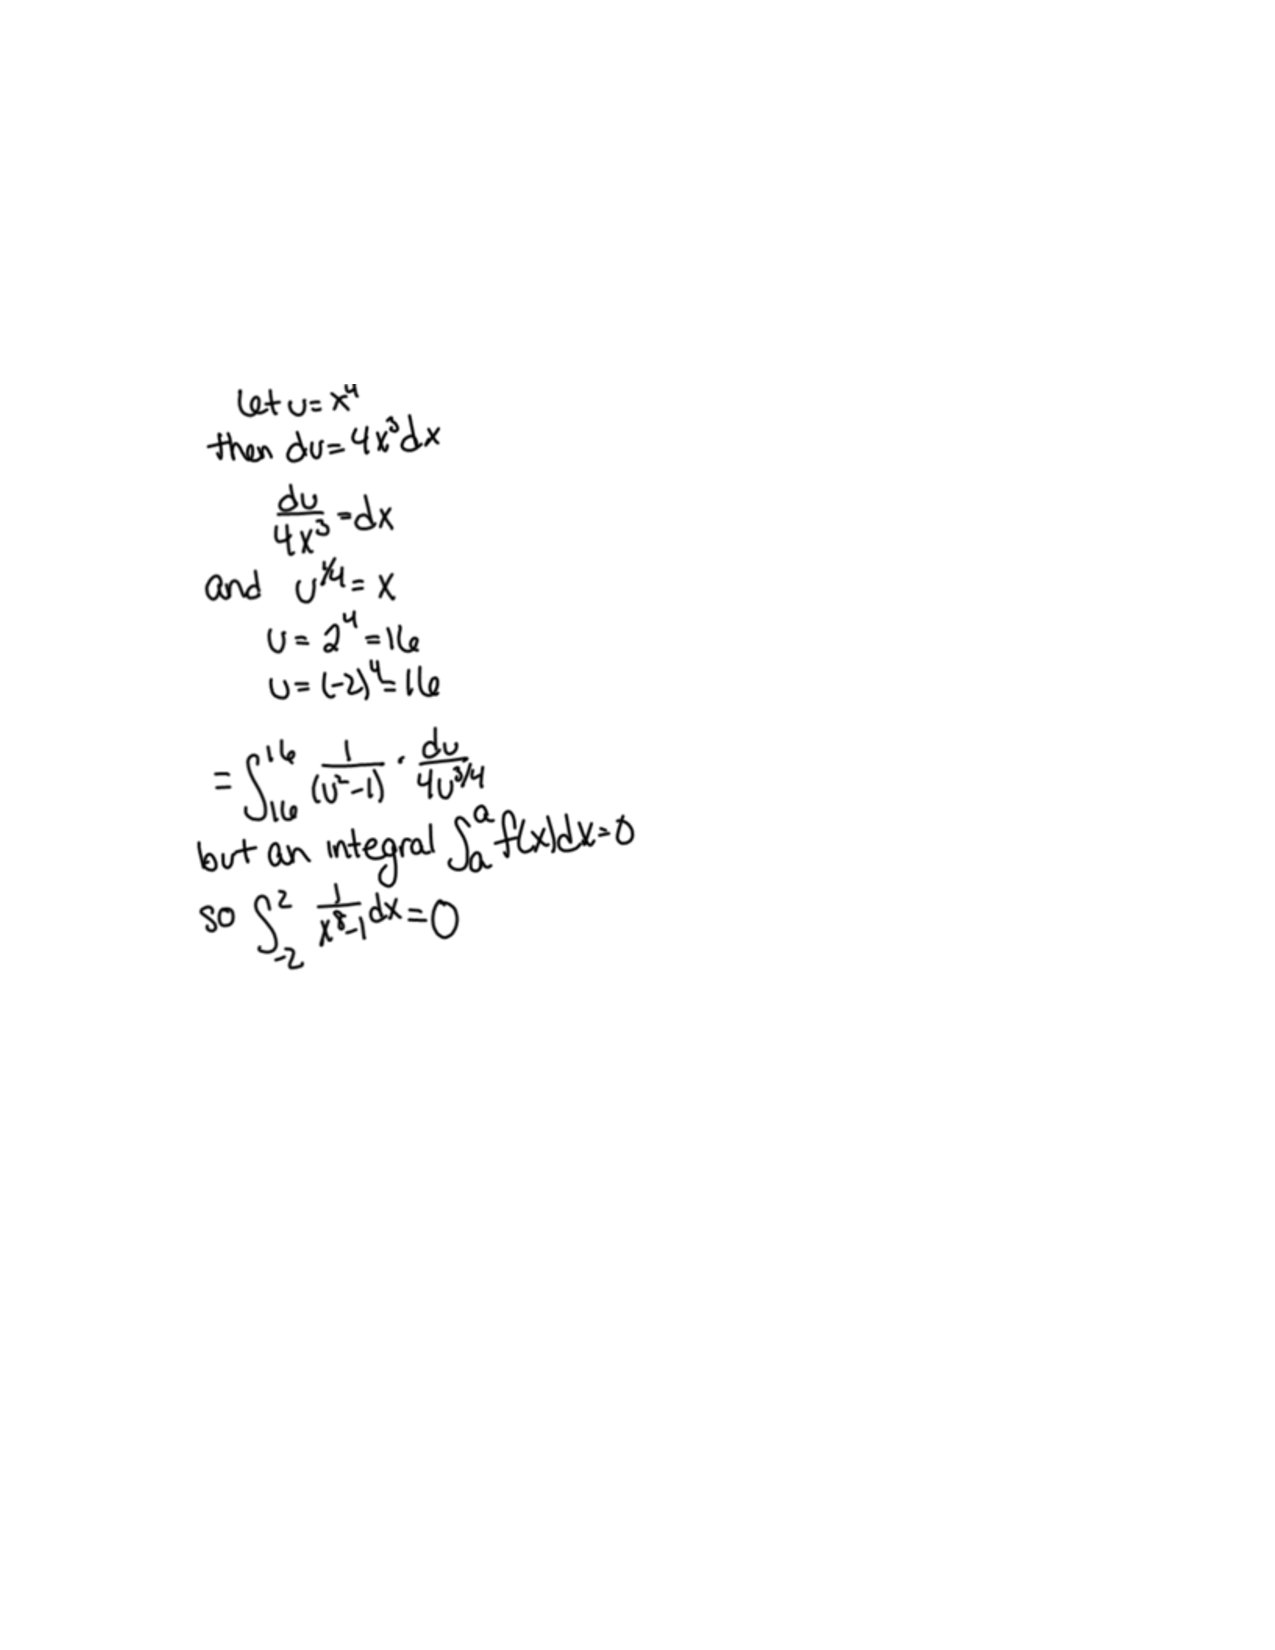
\includegraphics[trim= 170 420 250 180]{Figure1.pdf}
%\end{image}

%add a ``.'' below when used in a specific directory.
\newcommand{\RR}{\mathbb R}
\renewcommand{\d}{\,d}
\newcommand{\dd}[2][]{\frac{d #1}{d #2}}
\renewcommand{\l}{\ell}
\newcommand{\ddx}{\frac{d}{dx}}
\newcommand{\dfn}{\textbf}
\newcommand{\eval}[1]{\bigg[ #1 \bigg]}

\usepackage{multicol}

\renewenvironment{freeResponse}{
\ifhandout\setbox0\vbox\bgroup\else
\begin{trivlist}\item[\hskip \labelsep\bfseries Solution:\hspace{2ex}]
\fi}
{\ifhandout\egroup\else
\end{trivlist}
\fi} %% we can turn off input when making a master document

\title{Section 6.2: Regions Between Curves}  

\begin{document}
\begin{abstract}		\end{abstract}
\maketitle


%There was not a warm-up exercise for this specific section
\begin{comment}
\section{Warm up:}

	\begin{freeResponse}
	
	\end{freeResponse}
	
\begin{instructorNotes}

\end{instructorNotes}
\end{comment}







\section{Group work:}



%problem 1
\begin{problem}
Consider the region bounded by the curves $y=7x^2-12$ and $y=x^2-6x$.
	\begin{enumerate}
		\item  Draw a sketch of the graphs.
		\begin{freeResponse}
		Set the curves equal to each other to find the intersection points: \\
			$7x^2-12=x^2-6x\\
			6x^2+6x-12=0\\
			6(x^2+x-2)=0\\
			6(x-1)(x+2)=0\\
			x=1 \, or \, x=-2		$
			\begin{image}
			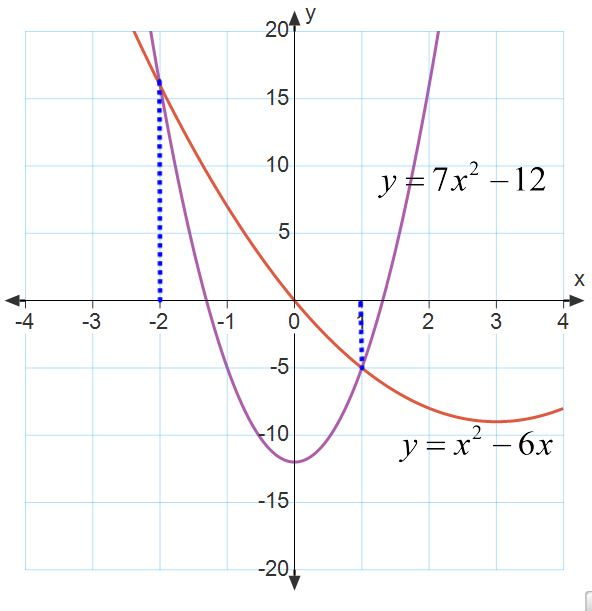
\includegraphics[scale=0.5]{Figure6-2-2new.jpg}
			\end{image}
		\end{freeResponse}
		\newpage
		\item  Find the area between these curves.
		\begin{freeResponse}
		By the solution to part (a), we know that these two curves intersect at $x=-2, 1$.  
		By checking the point $x=0$ (or by looking at the graph from part (a)) we see that $y=7x^2-12  \leq y=x^2-6x$ on the interval $[-2,1]$. Said another way, y=$7x^2-12$ is on top and $ y=x^2-6x$ is on bottom on the interval [-2,1], and we will use "top - bottom" to find the area between the curves.  
		So the area between the curves is:
			\begin{align*}
			\int_{-2}^1 (x^2-6x) - (7x^2-12) \d x &= \int_{-2}^1 (-6x^2-6x+12) \d x  \\
			&= \eval{-2 x^3 -3 x^2 + 12x}_{-2}^1  \\
			&= \left(-2(1) -3(1) +12(1) \right) - \left(-2(-2)^3 -3(-2)^2 + 12(-2) \right)  \\
			&= 7 - (-20)  = 27
			\end{align*}
		\end{freeResponse}
		
		\item  Find the area of the region bounded by the curves $x=7y^2-12$ and $x=y^2-6y$.
		\begin{freeResponse}
		This region is exactly the same as the region from part (a), except it is rotated clockwise by $90^{\circ}$.  
		Since the area of a region does not change under rotation, we have that the area of the new region is still 27.
		\end{freeResponse}
		
		\item  Find the area of the region bounded by the curves  $y = 7x^2$ and $y=x^2 - 6x + 12$.
				\begin{freeResponse}
				The region bounded by the curves $y = 7x^2$ and $y=x^2 - 6x + 12$ is just the region in part (a) translated upward by 12 units.  
				Since the area of a region does not change under translation, we have that the area of the new region is still 27.  
				\end{freeResponse}
				
				

		
		\item  Find the area of the region bounded by the curves $y=7x^2-12$, $y=x^2-6x$, $x=0$, and $x=3$.
		\begin{freeResponse}
		\vspace{1mm}
			%\begin{image}
			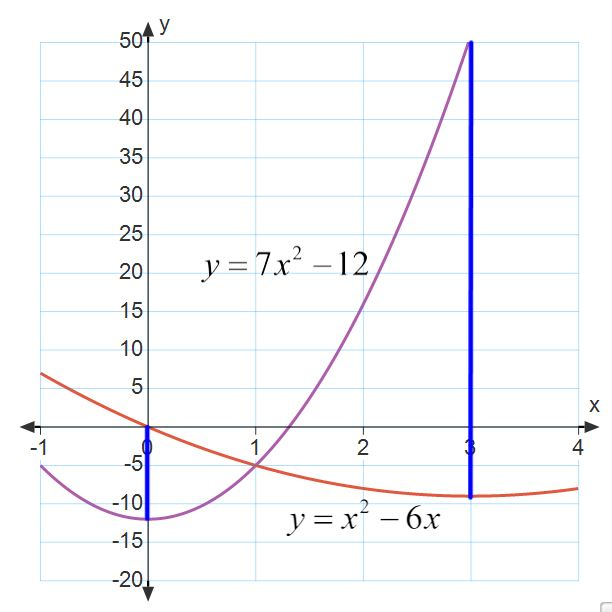
\includegraphics[scale=.5]{Figure6-2-3new.jpg}
			%\end{image}
		We already know that the graphs of the two functions intersect at the point $x=1$.  
		By checking the points $x=0$ and $x=3$ (or by looking at the graph above) we see that 
			\begin{align*}
			y=x^2-6x \geq y=7x^2-12 \quad \text{on} \quad [0,1]  \\
			y=7x^2-12 \geq y=x^2-6x \quad \text{on} \quad [1,3]
			\end{align*}
		Thus, the area between the curves is
			\begin{align*}
			&\int_0^1 (x^2-6x ) - (7x^2-1) \d x + \int_1^3 (7x^2-12) - (x^2-6x) \d x  \\
			&= \int_0^1 (-6^2 - 6x + 12) \d x + \int_1^3 (6x^2 + 6x - 12) \d x  \\
			&= \eval{-2 x^3 -3 x^2 + 12x}_0^1 + \eval{2 x^3 + 3 x^2 - 12x}_1^3  \\
			&= \left[ \left(- 2 -3 + 12 \right) - 0 \right] + \left[ \left( 2 (27) +3 (9) - 12(3) \right) - \left(  2 +3 - 12 \right) \right]  \\
			&=  7+ 54 + 27 -36 +7 = 59
			\end{align*}
		\end{freeResponse}
		
	\end{enumerate}
	
\end{problem}

\begin{instructorNotes}
Have the students do (a) and (b), and then have a group present.  
Afterwards, discuss the variations (c) and (d) as a whole class.
\end{instructorNotes}





\newpage

%problem 2
\begin{problem}
Set up two different integrals that compute the area of the region bounded by the curves  $x=y^2$ and $y=6-x$ (and be sure to draw a sketch of the graphs).
	
				\begin{freeResponse} 
				\textbf{ In terms of $y$:}\\
				First we find the intersection points:\\
				$y^2=6-y\\
				y^2+y-6=0\\
				(y+3)(y-2)=0\\
				y=-3 \, or \, y=2$
			\begin{image}
			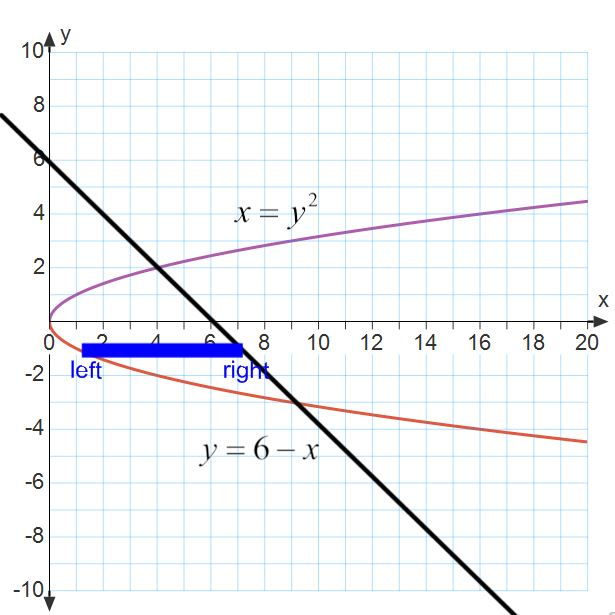
\includegraphics[scale=0.5]{Figure6-2-4new.jpg}
			\end{image}
		Thus,
		\[
		\text{{\color{red} Area of region}} =  \int_{-3}^2 [(6-y) - y^2] \d y .
		\]
		
		\textbf{In terms of $x$:}\\
		We need to rewrite $x=y^2$ as the two functions $y=\sqrt{x}$ and $y=-\sqrt{x}$.  Then,
		we need two integrals because the top function changes where $y=\sqrt{x}$ intersects $y=6-x$.
		We also need to find our intersection points in terms of $x$.  Since we already know the $y$-values of the points, 
		we can plug the y-values into either function to get the $x$-values:\\
		$x=6-y\\
		x(2)=6-2=4\\
		x(-3)=6-(-3)=9$\\
		\begin{image}
			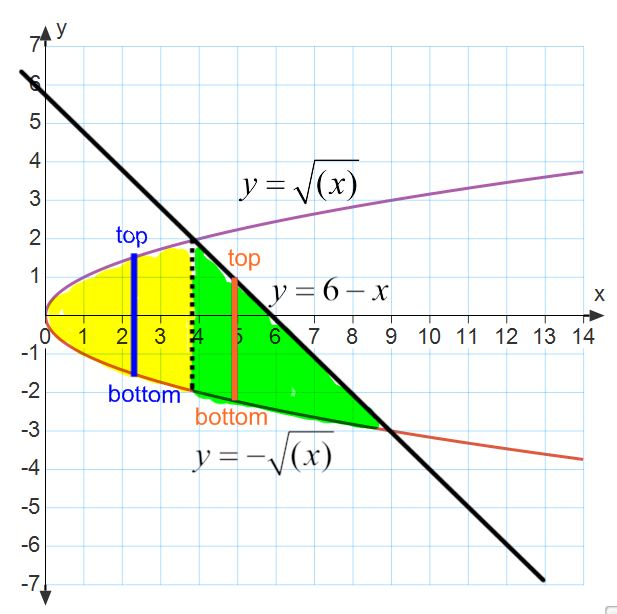
\includegraphics[scale=0.5]{Figure6-2-4new2.jpg}
			\end{image}
			Thus,
		\[
		\text{{\color{red} Area of region}} =  \int_0^4 (\sqrt{x} - (-\sqrt{x})) \d x + \int_4^9 ((6-x)-(-\sqrt{x})) \d x .
		\]
		
		\end{freeResponse}
		


\end{problem}

\begin{instructorNotes}
Split (a) and (b) among the groups.  
Note that (a) should be set up in terms of $y$ while (b) should be set up in terms of $x$.  
Have groups present their solutions.  
Discuss with the students factors to consider when deciding whether to integrate in terms of $x$ or $y$.
\end{instructorNotes}



\newpage



%problem 3
\begin{problem}
Two runners ($A$ and $B$) run in a race in which the winner runs the greater distance after $4$ minutes.  
The runners' respective velocities are
\[
v_A(t) = \frac{1}{3} t^2	\qquad	 v_B(t) = t
\]
The graphs of the runners' velocities is given below.  

\begin{image}
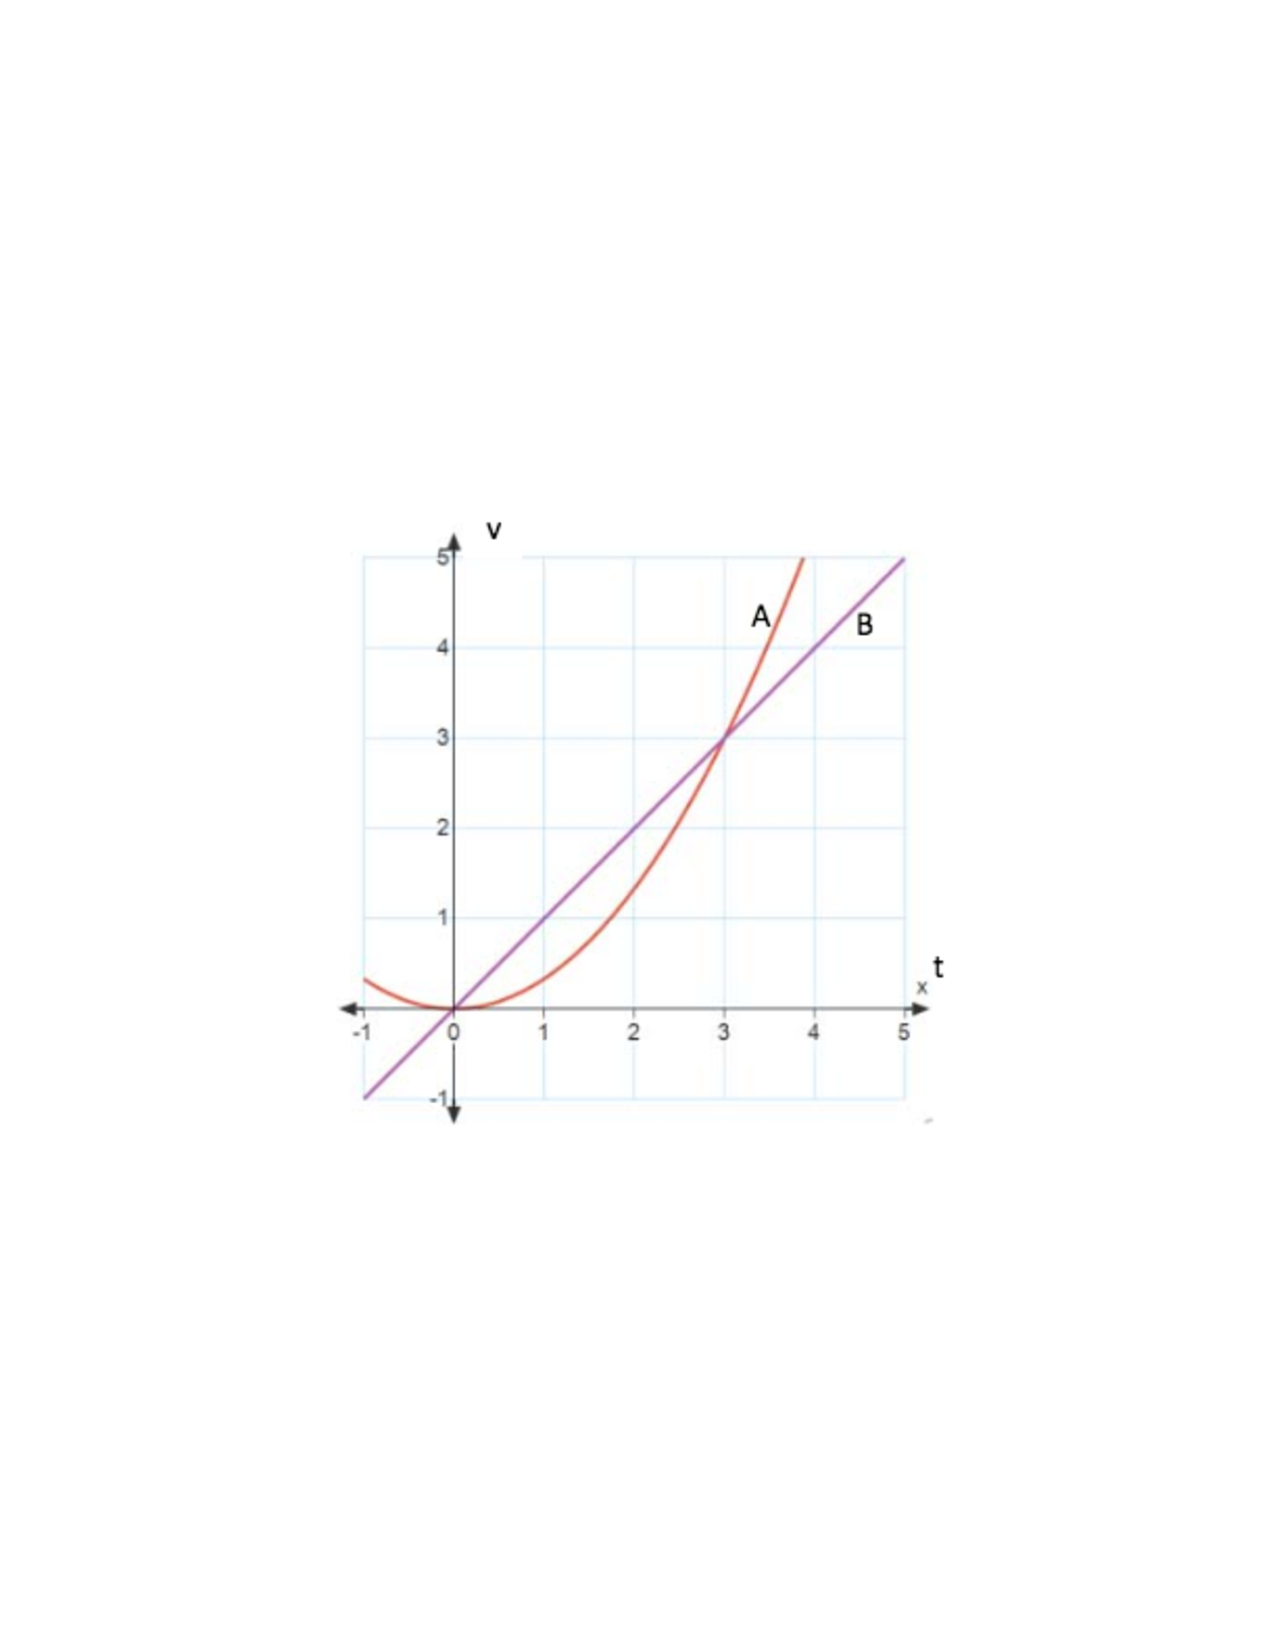
\includegraphics[trim= 270 250 250 250]{Figure6-2-1.pdf}
\end{image}

	\begin{enumerate}
		\item  Who is running faster $2$ minutes into the race?
		\begin{freeResponse}
		$v_A(2) = \frac{4}{3}$ and $v_B(2) = 2$.  
		So $B$ is running faster at the $2$ minute mark of the race.
		\end{freeResponse}
		
		\item  Who is winning the race $2$ minutes into the race (and by how much)?
		\begin{freeResponse}
		The distance that $A$ covers in the first $2$ minutes is
		\[
		\int_0^2 v_A(t) \d t = \int_0^2 \frac{1}{3} t^2 \d t = \eval{\frac{1}{9} t^3}_0^2 = \frac{8}{9}.
		\]
		The distance that $B$ covers in the first $2$ minutes is
		\[
		\int_0^2 v_B(t) \d t = \int_0^2 t \d t = \eval{\frac{1}{2} t^2}_0^2 = 2.
		\]
		So $B$ is winning after $2$ minutes.
		
		$B$ is winning by $2 - \frac{8}{9} = \frac{10}{9}$.  
		This could also be calculated by
		\[
		\int_0^2 (v_B(t) - v_A(t)) \d t.
		\]
			\begin{image}
			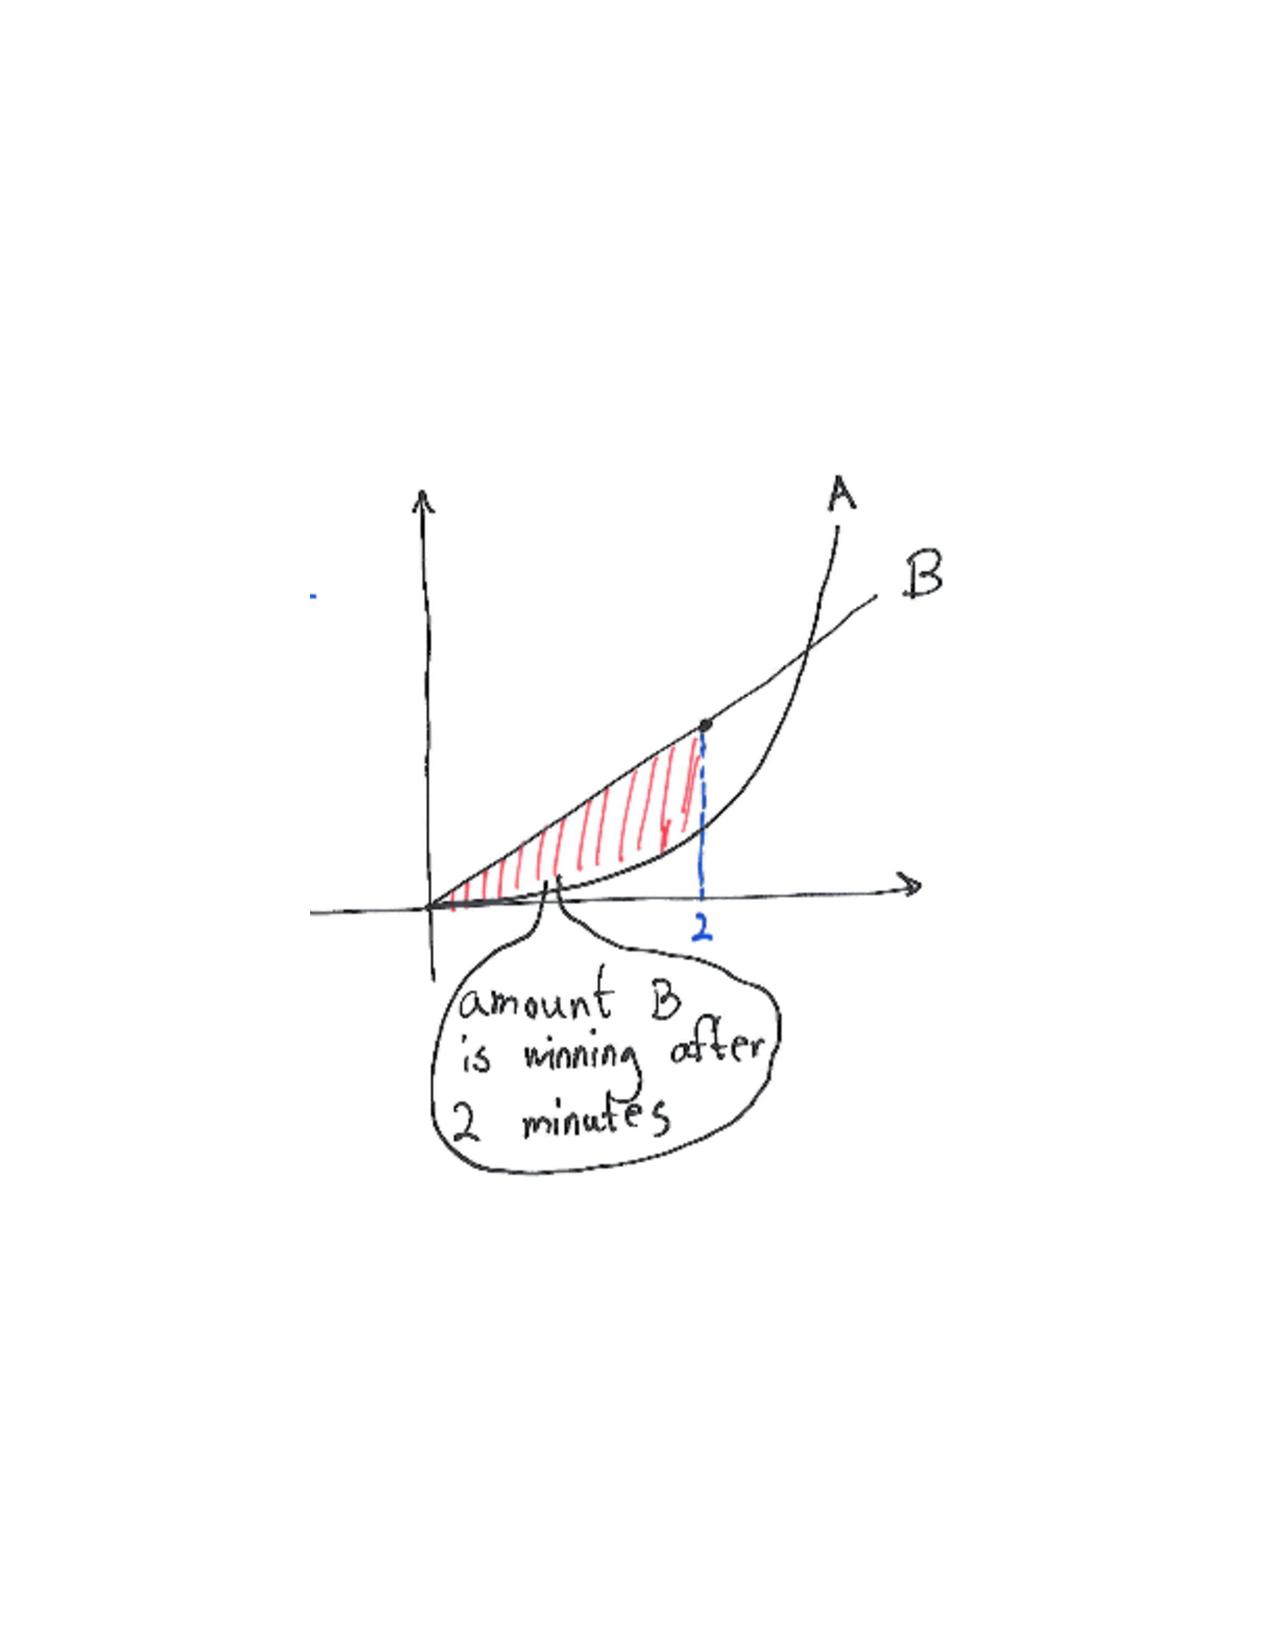
\includegraphics[trim= 130 230 100 230,scale=0.8]{Figure6-2-6.pdf}
			\end{image}
		\end{freeResponse}
		
		\item  What special event occurs $3$ minutes into the race?
		\begin{freeResponse}
		Runner $A$ matches runner $B$'s velocity.  
		ie, $v_A(3) = v_B(3)$.  
		\end{freeResponse}
		
		\item  Who wins the race (and by how much)?
		\begin{freeResponse}
		The distance that $A$ covers is
		\[
		\int_0^4 v_A(t) \d t = \int_0^4 \frac{1}{3} t^2 \d t = \eval{\frac{1}{9} t^3}_0^4 = \frac{64}{9} = 7.\overline{1}.
		\]
		The distance that $B$ covers is
		\[
		\int_0^4 v_B(t) \d t = \int_0^4 t \d t = \eval{\frac{1}{2} t^2}_0^4 = 8.
		\]
		So runner $B$ wins.  The amount that $B$ wins by is
		\[
		8 - \frac{64}{9} = \frac{8}{9}.
		\]
		This could have also been computed by
		\[
		\int_0^4 (v_B(t) - v_A(t)) \d t.
		\]
			\begin{image}
			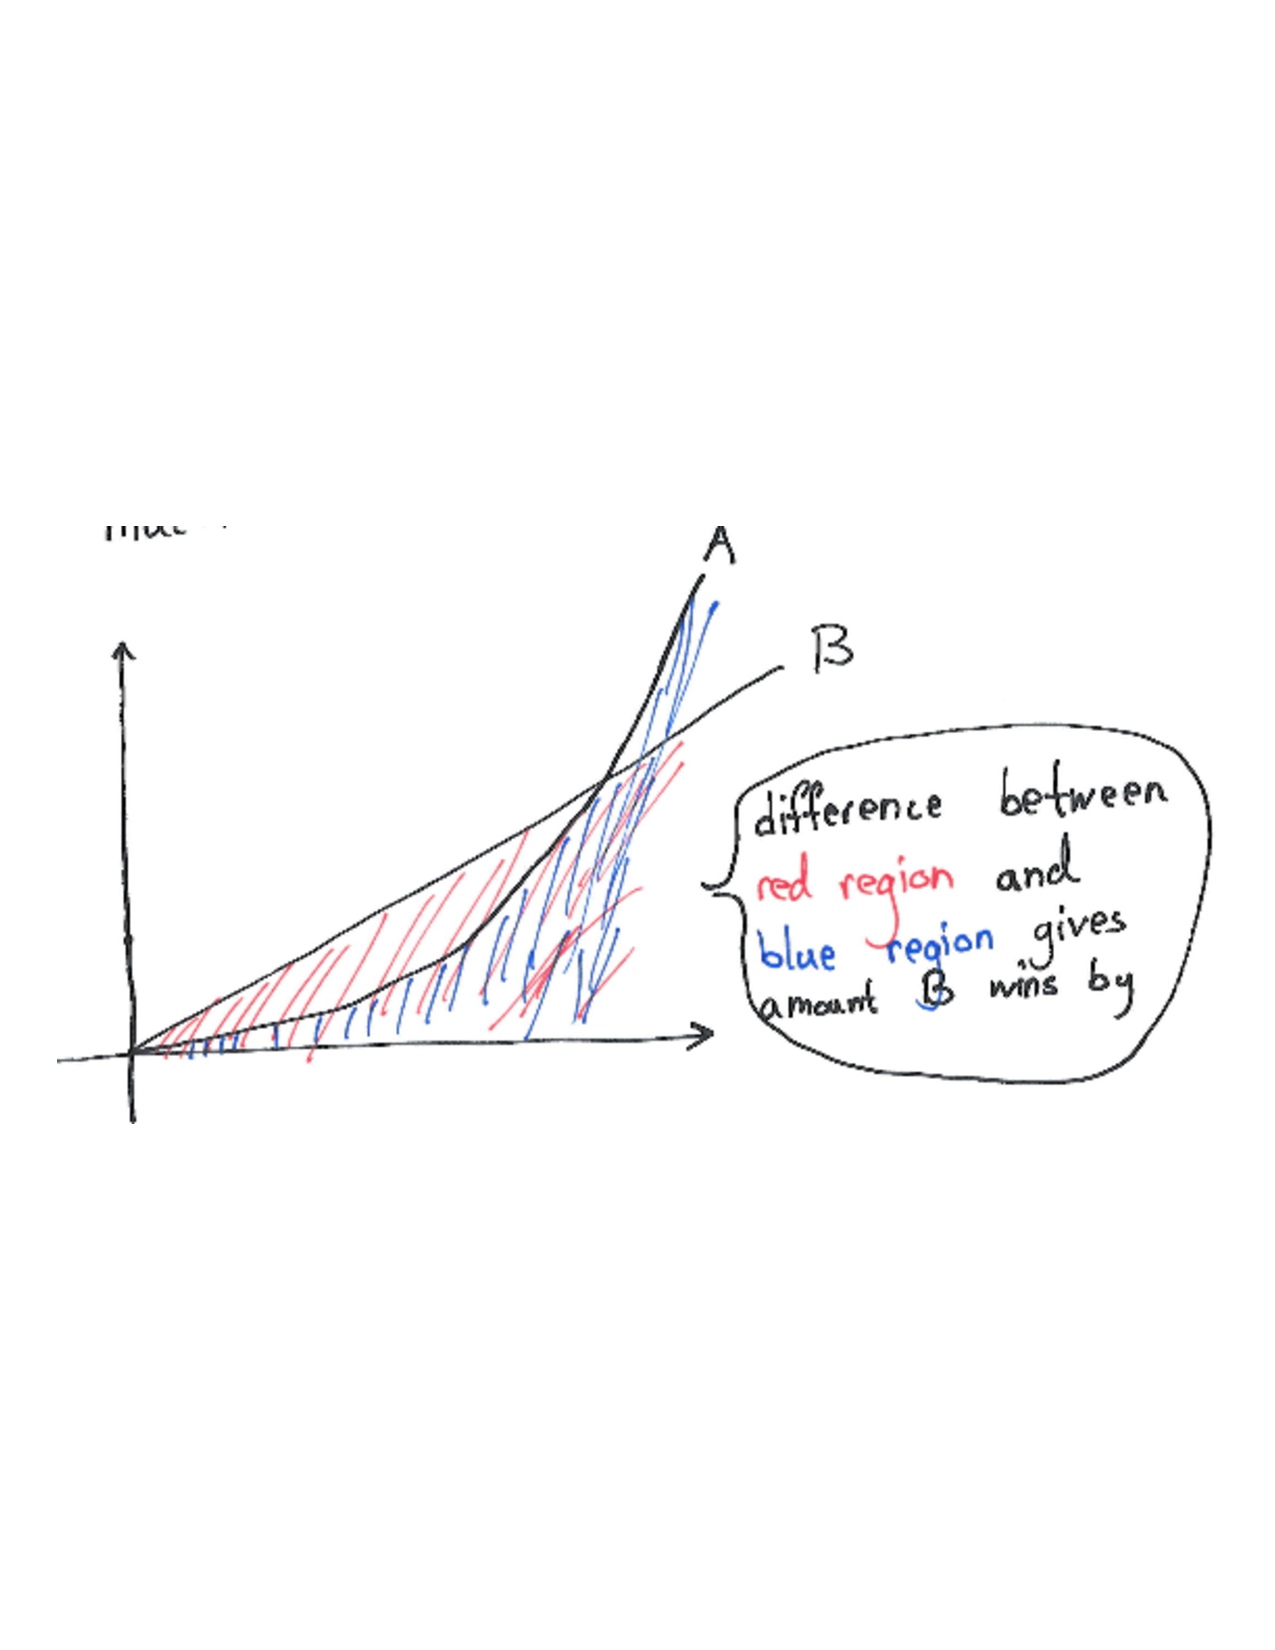
\includegraphics[trim= 130 250 100 250,scale=0.6]{Figure6-2-7.pdf}
			\end{image}
		\end{freeResponse}
		
		\end{enumerate}

\end{problem}

\begin{instructorNotes}
Do this problem as a class discussion.  
The main point is to have students identify how each of the questions relates to the graph of the velocity functions.
\end{instructorNotes}
















	
	
	
	
	
	
	
	
	

	










								
				
				
	














\end{document} 


















